\documentclass[11pt]{article}

\usepackage{lscape,color}
\usepackage[normalem]{ulem}

\topmargin -0.75truein
\oddsidemargin -0.4truein
\textheight 9.25truein
\textwidth 6.7truein
\hbadness=10001
\hfuzz=200pt

\begin{document}
\newcommand{\be}{\begin{enumerate}}
\newcommand{\ee}{\end{enumerate}}
\newcommand{\bc}{\begin{center}}
\newcommand{\ec}{\end{center}}
\newcommand{\bi}{\begin{itemize}}
\newcommand{\ei}{\end{itemize}}
\newcommand{\bd}{\begin{description}}
\newcommand{\ed}{\end{description}}
\newcommand{\bt}{\begin{tabbing}}
\newcommand{\et}{\end{tabbing}}
\newcommand{\eg}{{\it e.g.~}}
\newcommand{\ie}{{\it i.e.~}}
\newcommand{\ul}{\underline}
\newcommand{\axaf}{{\em AXAF}}
\def\la{\hbox{\rlap{$<$}\lower0.5ex\hbox{$\sim$}\ }}

\centerline{\large {\bf \textcolor{red}{5.9\_V2.2} SWITCH FROM DEA A TO DEA B }}
\vspace{0.25in}

\noindent{\it Last Revised: June 17, 2016}\\
\noindent{\bf Filename: switch\_deaa\_b} \\


\noindent{\bf BRIEF FUNCTIONAL DESCRIPTION:}\\

\textcolor{red}{This is a contingency procedure to switch from powering the DEA from the
A-side of the PSMC to powering it from the B-side.
After switching DEA input power and reestablishing control of the
focal plane heaters, the magnetic relays that control pairs
of video boards are thrown one at a time,
and those two video boards are powered up separately,
while verifying that the PSMC doesn't report a current overflow.}

\vspace{0.15in}

\noindent The sequence of actions will be:
{\color{red}
\begin{itemize}
\item Power down the video boards (skip if not powered)

\item Turn off and disable the DEA side A power supply (skip if not enabled and on)

\item Verify that all DEA side B heaters are off and disabled

\item Enable and turn on the DEA side B power supply

\item Perform a warm boot of the active BEP

\item Start DEA interface housekeeping

\item Enable DEA-B to assume control of the focal plane temperature
by commanding it to $-122^\circ$~C and then to $-120^\circ$~C

\item Switch the video board relays one at a time,
wait for PSMC telemetry verifiers to refresh,
and verify that DEA-B hasn't powered down due to an overcurrent
or overvoltage condition

\item After switching each pair of video boards,
power up each of the two boards, waiting for PSMC telemetry verifiers to refresh,
and verifying that DEA-B hasn't powered down due to an overcurrent
or overvoltage condition

\item Power down all video boards

\item Dump the system configuration table
\end{itemize}
}

\vspace{0.15in}

\noindent{\bf ASSUMED INSTRUMENT STATE:}
\bi
\item Assumes that DPA A and/or DPA B is on and that the flight SW is running.
\item \sout{Assumes that DEA A is on.}
\ei

\vspace{0.15in}

\noindent{\bf SPECIAL INITIAL CONDITIONS:}
{\color{red}
\bi
\item Assumes that telemetry is in Format 1 or 2.
\item Assumes that neither the bakeout heater nor the detector housing heater is
being powered by DEA-B. If they are, switch them off and, if the procedure ends
with the DEA powered from DEA-B, consider enabling and turning them on again
on DEA-A.
\ei}

\newpage

\noindent{\bf CHANGE HISTORY:}

\bd
\item {\bf Version 1.2}
\bi
\item added a new step 1 to start a DEA HKP run if necessary
\item changed HW TLM verifiers to check state of DEA A and DEA B in
steps 2.1 and 3.2
\item added a new step 5 to warmboot the active BEP
\item added a command in step 6 to set the focal plane temperature to
$-120^\circ$~C
\item added operational constraint/caution that the B side does not
produce the telltales to verify the state of the relays
\ei

\item {\bf Version 2.0}
\bi
\item ACIS Team signed-off version
\item changed expected value of ``1STAT7ST'' in step 5.6
\ei

\item {\bf Version 2.1}
\bi
\item changed comment in step 1.2 to read ``check FP temp''
\item changed telemetry verified in step 5.5 to read ``version=??''
  and changed comment to read ``version \# depends on loaded patches,
  if any''
\item changed expected value of ``1STAT7ST'' in step 5.6
\item changed command in step 6.2 to WSFTNEG121
\item added to ``Assumed Instrument State'', ``Assumes DEA A is on''
\ei

{\color{red}
\item {\bf Version 2.2}
\bi
\item added explicit step to verify that 28V heaters are off before powering DEA-B
\item replaced warm boot with FP temperature changes
\item replaced command to switch all 5 relays simultaneously with 5 sets of 3 commands:
a command to switch one of the relays,
followed by a pair of commands to power up each of the two boards controlled by that relay
\item added command to power up 6 FEPs
\item added bias-only run to acquire housekeeping from ACIS-I boards
\item added bias-only run to acquire housekeeping from ACIS-S boards
\item added command to power down all video boards
\ei}
\ed

\newpage\
\vspace{0.4\textheight}
\bc This page is intentionally blank \ec

\newcommand{\tablecaptiontext}{SWITCH FROM DEA A TO DEA B}
\documentclass[11pt]{article}

\usepackage{lscape,color}
\usepackage[normalem]{ulem}
\usepackage{url}
\usepackage{graphicx}

\topmargin -0.75truein
\oddsidemargin -0.4truein
\textheight 9.25truein
\textwidth 6.7truein
\hbadness=10001
\hfuzz=200pt

\begin{document}
\newcommand{\be}{\begin{enumerate}}
\newcommand{\ee}{\end{enumerate}}
\newcommand{\bc}{\begin{center}}
\newcommand{\ec}{\end{center}}
\newcommand{\bi}{\begin{itemize}}
\newcommand{\ei}{\end{itemize}}
\newcommand{\bd}{\begin{description}}
\newcommand{\ed}{\end{description}}
\newcommand{\bt}{\begin{tabbing}}
\newcommand{\et}{\end{tabbing}}
\newcommand{\eg}{{\it e.g.~}}
\newcommand{\ie}{{\it i.e.~}}
\newcommand{\ul}{\underline}
\newcommand{\axaf}{{\em AXAF}}
\def\la{\hbox{\rlap{$<$}\lower0.5ex\hbox{$\sim$}\ }}

\centerline{\large {\bf 5.9\_V2.2 SWITCH FROM DEA A TO DEA B }}
\vspace{0.25in}

\noindent{\it Last Revised: December 6, 2017}\\
\noindent{\bf Filename: switch\_deaa\_b} \\


\noindent{\bf BRIEF FUNCTIONAL DESCRIPTION:}\\

This is a contingency procedure to switch from powering the DEA 
from the side A power supply board to the side B power supply board inside 
the PSMC. After switching DEA input power and reestablishing control of the
focal plane heaters, the magnetic relays that control pairs of video boards 
are thrown one at a time, and those two video boards are powered up separately,
while verifying that the PSMC doesn't report a current overflow.

Once 10 video boards have been powered up, power up 6 FEPs and execute bias-only 
runs in the ACIS-I and ACIS-S configurations to generate accurate video-board 
housekeeping. Once finished, power down all FEPs and video boards.

\vspace{0.15in}

\noindent The sequence of actions will be:
\begin{itemize}
\item Power down the video boards (skip if not powered)
\vspace{-0.10in}
\item Turn off and disable the DEA side A power supply (skip if not enabled and on)
\vspace{-0.10in}
\item Verify that DEA side A is off and disabled
\vspace{-0.10in}
\item Verify that all DEA side B heaters are off and disabled
\vspace{-0.10in}
\item Enable and turn on the DEA side B power supply
\vspace{-0.10in}
\item Verify that DEA side A is off and disabled
\vspace{-0.10in}
\item Perform a warm boot of the active BEP
\vspace{-0.10in}
\item Start DEA interface housekeeping
\vspace{-0.10in}
\item Enable DEA-B to assume control of the focal plane temperature
by commanding it to $-122^\circ$~C and then to $-120^\circ$~C
\vspace{-0.10in}
\item Switch the video board relays one at a time,
wait for PSMC telemetry verifiers to refresh,
and verify that DEA-B hasn't powered down due to an overcurrent
or overvoltage condition
\vspace{-0.10in}
\item After switching each pair of video boards,
power up each of the two boards, waiting for PSMC telemetry verifiers to 
refresh, and verifying that DEA-B hasn't powered down due to an overcurrent
or overvoltage condition
\vspace{-0.10in}
\item Power up 6 FEPs
\vspace{-0.10in}
\item Execute a bias-only science run in the ACIS-I configuration.
\vspace{-0.10in}
\item Execute a bias-only science run in the ACIS-S configuration.
\vspace{-0.10in}
\item Power down all FEPs and video boards
\vspace{-0.10in}
\item Dump the system configuration table
\end{itemize}

\vspace{0.15in}

\noindent{\bf ASSUMED INSTRUMENT STATE:}
\bi
\item Assumes that DPA A and/or DPA B is on, the flight SW is running and no 
science run is in progress.
\ei

\vspace{0.15in}

\noindent{\bf SPECIAL INITIAL CONDITIONS:}
\bi
\item Assumes that telemetry is in Format 1 or 2.
\item Assumes that neither the bakeout heater nor the detector housing heater is
being powered by DEA-B. If they are, switch them off and, if the procedure ends
with the DEA powered from DEA-B, consider enabling and turning them on again
on DEA-A.
\ei

\normalsize
\noindent {\bf OPERATIONAL CONSTRAINTS/CAUTIONS:} \\
\normalsize

In normal operations, only one side of the DEA should be powered on
(a) to prevent conflict for control of the focal plane temperature controller,
(b) to avoid excess current draw from the spacecraft,(c) to avoid over-heating
within the PSMC, and (d) to avoid placing a board 11 or 12 relay into the 
``magnetic neutral position''.

The DEA power status is normally indicated by the values of the 1DEPSA and
1DEPSB flags, which should not both be 1 simultaneously. Before sending the 
command to power on DEA B, the DEA Input Voltage B 1DE28BVO should 
be checked to make sure that DEA B is receiving power from the spacecraft.

The DEA input current monitors (1DEIC[AB]CU) are noisy.
To give an indication of what variation may be expected, figures 1 and 2
show the behavior of the A-side DEA current with a ten-sample running
average for two situations in which all video boards were powered down. Note that
when either side of the DEA is unpowered, the corresponding current monitor, 
1DEICACU for side A, or 1DEICBCU for side B, will be unreliable. They will read
16--18~A when unpowered, as of Telemetry Database (TDB) v14. This is expected and
not a problem.

If the DEA powers off unexpectedly during a bakeout, the FP bakeout 
heater will lose power and this heater will NOT be re-enabled when the DEA side B 
power is restored. Additional SW commands are necessary to activate the FP bakeout 
heater. The DH bakeout heater is unaffected by a power loss to the DEA and will 
therefore still be executing a bakeout if power is lost to the DEA.

The WSPOW commands in Step 8 of this procedure sequentially power up more and more 
video boards. Under some circumstances (e.g. looking for a board that may have a 
short or other anomaly), we may wish to skip one or more boards (e.g. suspected 
short circuit or other problem on one board). 

For more information about the relays, the DEA relays memo at 
\url{http://cxc.cfa.harvard.edu/acis/memos/DEA_Relay_Summary.html} should be 
consulted.

The parameters for the threshold crossings patch, txings, will revert to defaults 
when this is run. They should be restored to their desired values.

After successful execution, {\em the FP temperature control will be regulated at 
-119.7~$^\circ$C (if the spacecraft thermal environment allows), and DEA interface 
A/D will be in high-resolution mode.}

Skipping one or more boards in the power up sequence would require different 
WSPOW commands than are currently in this procedure.

Should any of the parts of step 8 fail or be intentionally skipped, so that less 
than 10 video boards remain powered up at the start of step 9, it will not be 
possible to obtain correct housekeeping from any of the video boards, so steps 
9-12 should be omitted.
\\

\newpage

\noindent{\bf CHANGE HISTORY:}

\bd
\item {\bf Version 1.2}
\bi
\item added a new step 1 to start a DEA HKP run if necessary
\item changed HW TLM verifiers to check state of DEA A and DEA B in
steps 2.1 and 3.2
\item added a new step 5 to warmboot the active BEP
\item added a command in step 6 to set the focal plane temperature to
$-120^\circ$~C
\item added operational constraint/caution that the B side does not
produce the telltales to verify the state of the relays
\ei

\item {\bf Version 2.0}
\bi
\item ACIS Team signed-off version
\item changed expected value of ``1STAT7ST'' in step 5.6
\ei

\item {\bf Version 2.1}
\bi
\item changed comment in step 1.2 to read ``check FP temp''
\item changed telemetry verified in step 5.5 to read ``version=??''
  and changed comment to read ``version \# depends on loaded patches,
  if any''
\item changed expected value of ``1STAT7ST'' in step 5.6
\item changed command in step 6.2 to WSFTNEG121
\item added to ``Assumed Instrument State'', ``Assumes DEA A is on''
\ei

\item {\bf Version 2.2}
\bi
\item added explicit steps to verify that DEA side A is off after sending the
disable and power off commands to side A and after DEA B is powered on
\item added explicit step to verify that the side B DH heater and the side B 
DH Bakeout heater are off before powering DEA-B
\item replaced command to switch all 5 relays simultaneously with 5 sets of 3 
commands: a command to switch one of the relays, followed by a pair of commands
to power up each of the two boards controlled by that relay
\item added command to power up 6 FEPs
\item added bias-only run to acquire housekeeping from ACIS-I boards
\item added bias-only run to acquire housekeeping from ACIS-S boards
\item added command to power down all video boards
\item added figures showing behavior of 1DEICACU
\item updated operational constraints and cautions text
and 
\ei
\ed

\begin{landscape}
\begin{figure}
\begin{center}
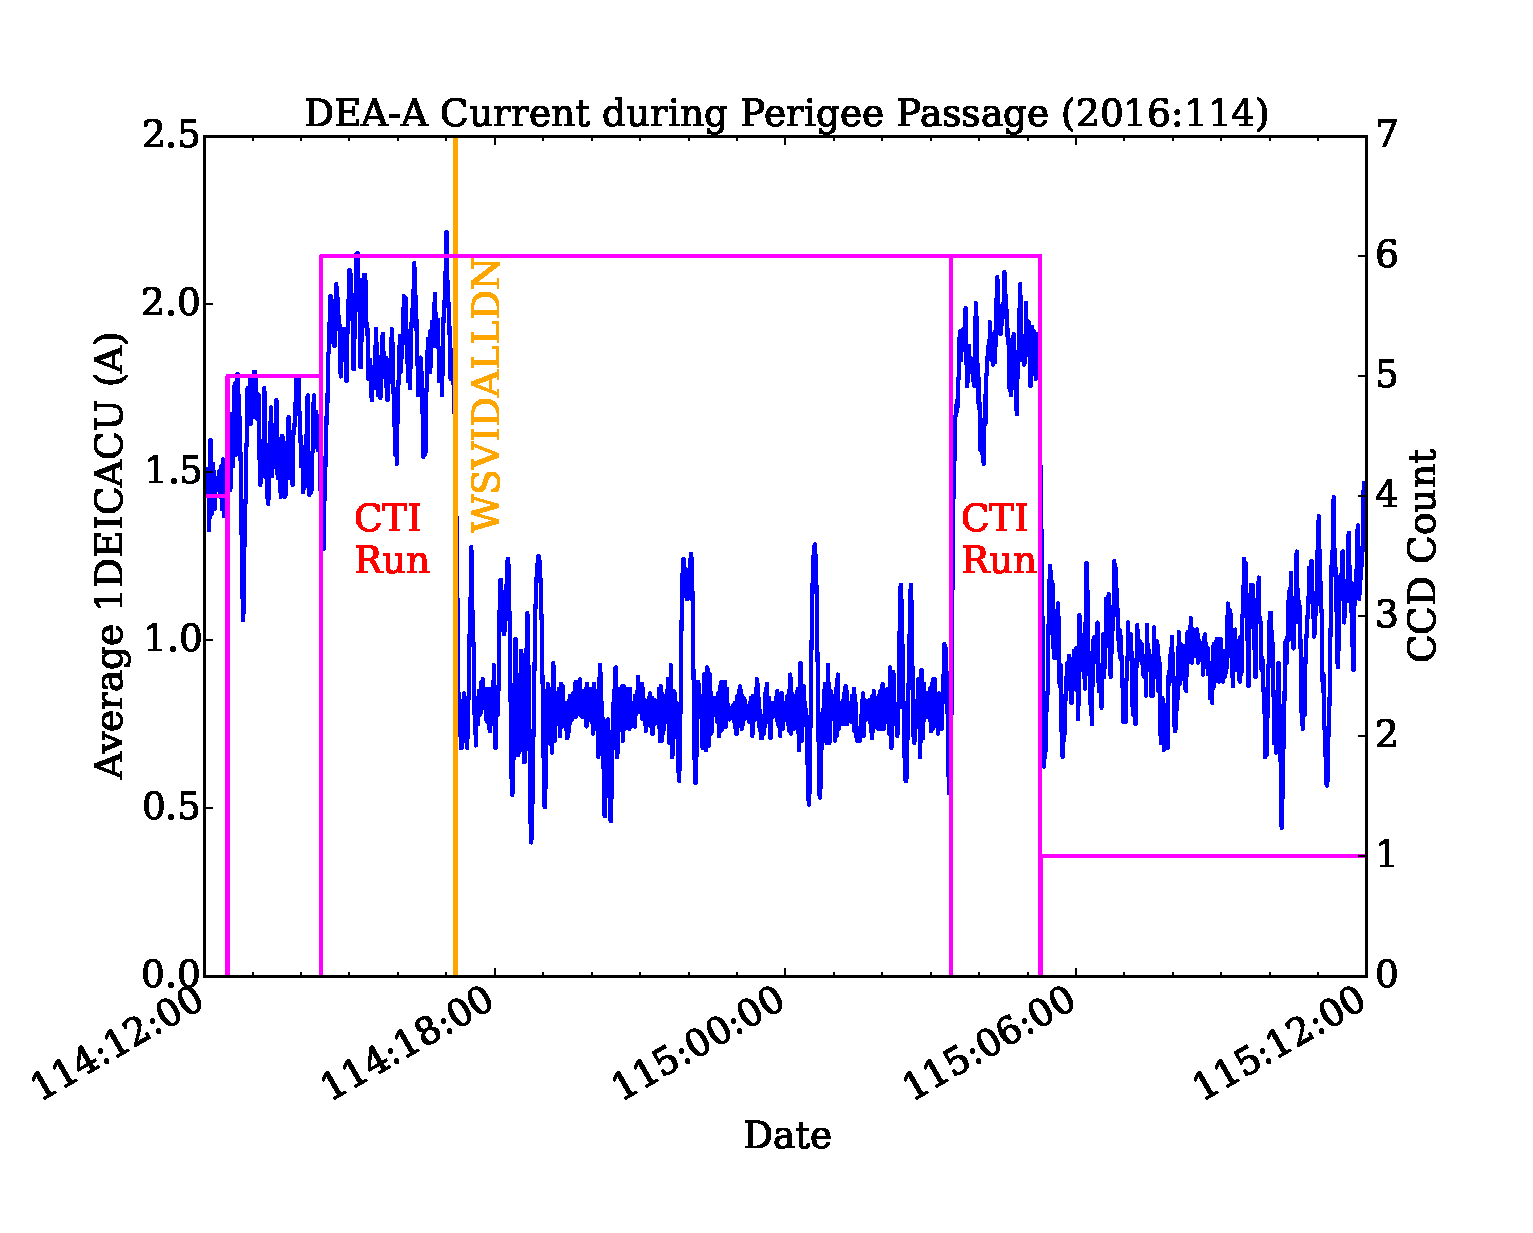
\includegraphics[width=1.2\textwidth]{switch_deaa_b_fig1.eps}
\caption{Average behavior of 1DEICACU during a perigee passage. All video boards
are powered off after the issuing of the WSVIDALLDN command, which is marked by
the orange line in the plot.}
\end{center}
\end{figure}
\end{landscape}
  
\begin{landscape}
\begin{figure}
\begin{center}
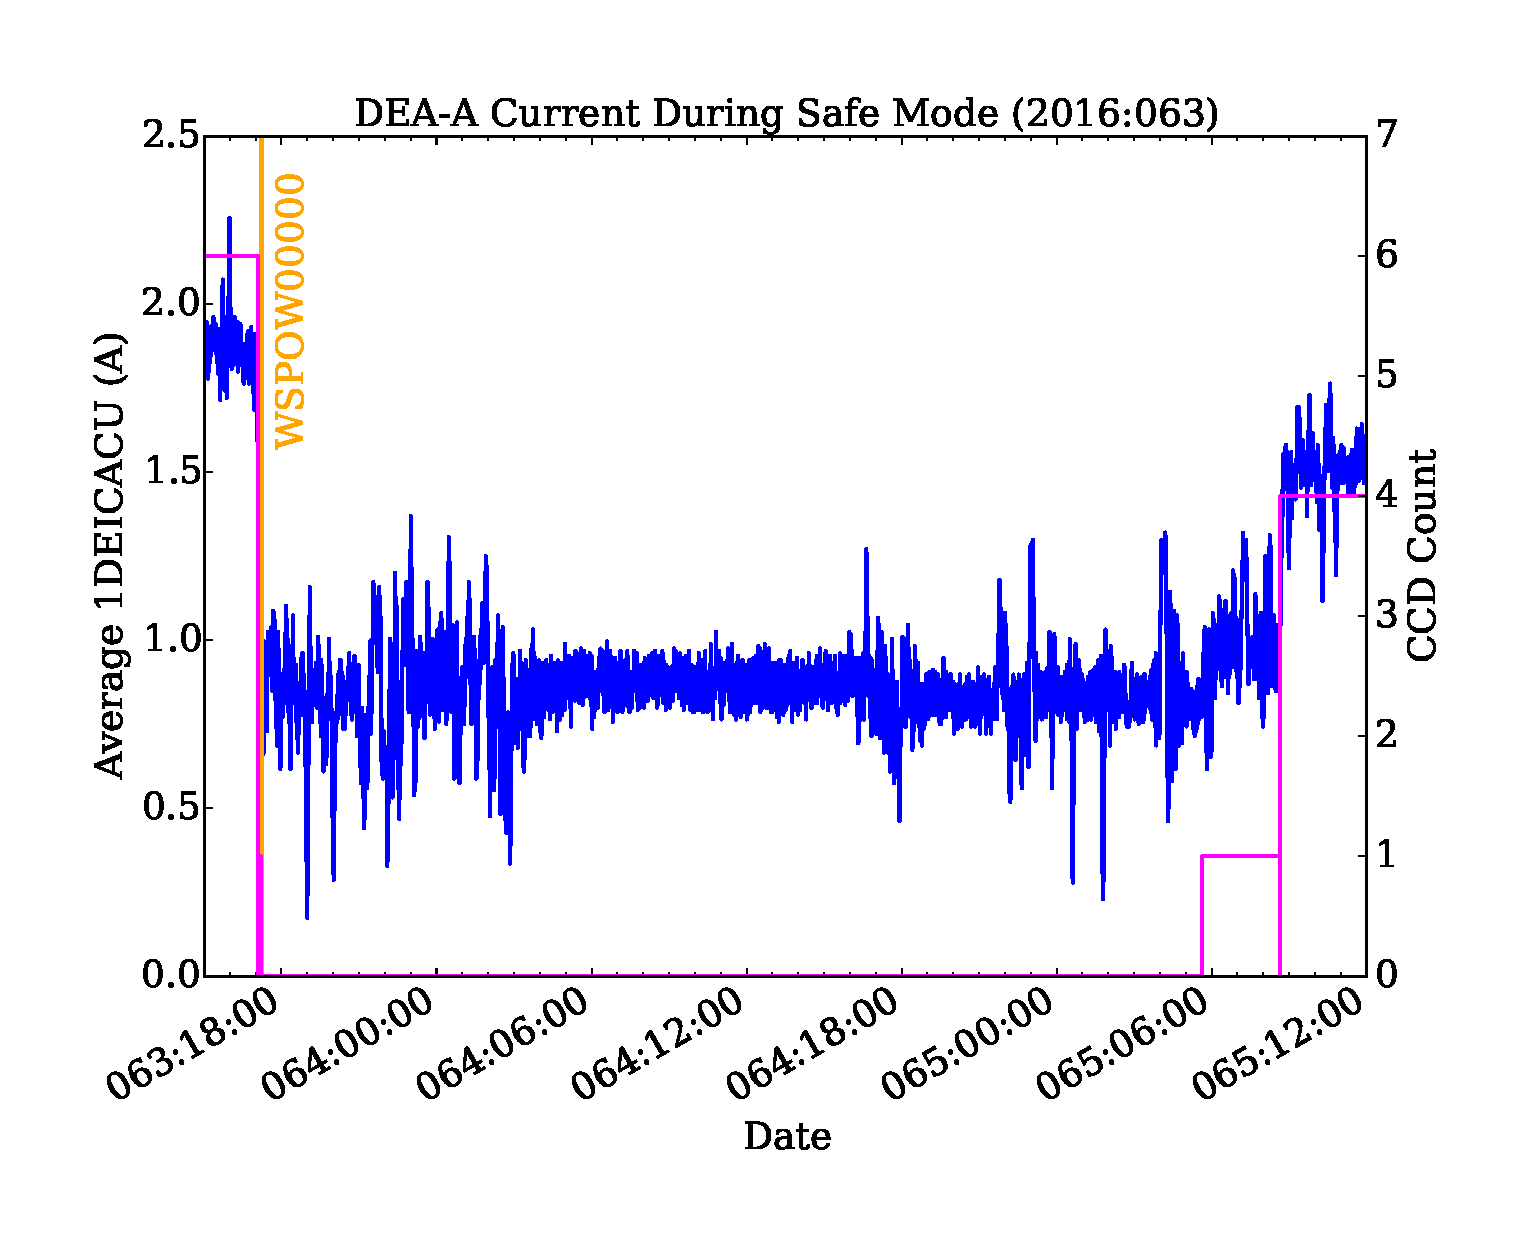
\includegraphics[width=1.2\textwidth]{switch_deaa_b_fig2.eps}
\caption{Average behavior of 1DEICACU during a safe mode. All video boards
are powered off after the issuing of the WSPOW00000 command, which is marked by
the orange line in the plot.}
\end{center}
\end{figure}
\end{landscape}
  
\newcommand{\tablecaptiontext}{SWITCH FROM DEA A TO DEA B}
\documentclass[11pt]{article}

\usepackage{lscape,color}
\usepackage[normalem]{ulem}
\usepackage{url}
\usepackage{graphicx}

\topmargin -0.75truein
\oddsidemargin -0.4truein
\textheight 9.25truein
\textwidth 6.7truein
\hbadness=10001
\hfuzz=200pt

\begin{document}
\newcommand{\be}{\begin{enumerate}}
\newcommand{\ee}{\end{enumerate}}
\newcommand{\bc}{\begin{center}}
\newcommand{\ec}{\end{center}}
\newcommand{\bi}{\begin{itemize}}
\newcommand{\ei}{\end{itemize}}
\newcommand{\bd}{\begin{description}}
\newcommand{\ed}{\end{description}}
\newcommand{\bt}{\begin{tabbing}}
\newcommand{\et}{\end{tabbing}}
\newcommand{\eg}{{\it e.g.~}}
\newcommand{\ie}{{\it i.e.~}}
\newcommand{\ul}{\underline}
\newcommand{\axaf}{{\em AXAF}}
\def\la{\hbox{\rlap{$<$}\lower0.5ex\hbox{$\sim$}\ }}

\centerline{\large {\bf 5.9\_V2.2 SWITCH FROM DEA A TO DEA B }}
\vspace{0.25in}

\noindent{\it Last Revised: December 6, 2017}\\
\noindent{\bf Filename: switch\_deaa\_b} \\


\noindent{\bf BRIEF FUNCTIONAL DESCRIPTION:}\\

This is a contingency procedure to switch from powering the DEA 
from the side A power supply board to the side B power supply board inside 
the PSMC. After switching DEA input power and reestablishing control of the
focal plane heaters, the magnetic relays that control pairs of video boards 
are thrown one at a time, and those two video boards are powered up separately,
while verifying that the PSMC doesn't report a current overflow.

Once 10 video boards have been powered up, power up 6 FEPs and execute bias-only 
runs in the ACIS-I and ACIS-S configurations to generate accurate video-board 
housekeeping. Once finished, power down all FEPs and video boards.

\vspace{0.15in}

\noindent The sequence of actions will be:
\begin{itemize}
\item Power down the video boards (skip if not powered)
\vspace{-0.10in}
\item Turn off and disable the DEA side A power supply (skip if not enabled and on)
\vspace{-0.10in}
\item Verify that DEA side A is off and disabled
\vspace{-0.10in}
\item Verify that all DEA side B heaters are off and disabled
\vspace{-0.10in}
\item Enable and turn on the DEA side B power supply
\vspace{-0.10in}
\item Verify that DEA side A is off and disabled
\vspace{-0.10in}
\item Perform a warm boot of the active BEP
\vspace{-0.10in}
\item Start DEA interface housekeeping
\vspace{-0.10in}
\item Enable DEA-B to assume control of the focal plane temperature
by commanding it to $-122^\circ$~C and then to $-120^\circ$~C
\vspace{-0.10in}
\item Switch the video board relays one at a time,
wait for PSMC telemetry verifiers to refresh,
and verify that DEA-B hasn't powered down due to an overcurrent
or overvoltage condition
\vspace{-0.10in}
\item After switching each pair of video boards,
power up each of the two boards, waiting for PSMC telemetry verifiers to 
refresh, and verifying that DEA-B hasn't powered down due to an overcurrent
or overvoltage condition
\vspace{-0.10in}
\item Power up 6 FEPs
\vspace{-0.10in}
\item Execute a bias-only science run in the ACIS-I configuration.
\vspace{-0.10in}
\item Execute a bias-only science run in the ACIS-S configuration.
\vspace{-0.10in}
\item Power down all FEPs and video boards
\vspace{-0.10in}
\item Dump the system configuration table
\end{itemize}

\vspace{0.15in}

\noindent{\bf ASSUMED INSTRUMENT STATE:}
\bi
\item Assumes that DPA A and/or DPA B is on, the flight SW is running and no 
science run is in progress.
\ei

\vspace{0.15in}

\noindent{\bf SPECIAL INITIAL CONDITIONS:}
\bi
\item Assumes that telemetry is in Format 1 or 2.
\item Assumes that neither the bakeout heater nor the detector housing heater is
being powered by DEA-B. If they are, switch them off and, if the procedure ends
with the DEA powered from DEA-B, consider enabling and turning them on again
on DEA-A.
\ei

\normalsize
\noindent {\bf OPERATIONAL CONSTRAINTS/CAUTIONS:} \\
\normalsize

In normal operations, only one side of the DEA should be powered on
(a) to prevent conflict for control of the focal plane temperature controller,
(b) to avoid excess current draw from the spacecraft,(c) to avoid over-heating
within the PSMC, and (d) to avoid placing a board 11 or 12 relay into the 
``magnetic neutral position''.

The DEA power status is normally indicated by the values of the 1DEPSA and
1DEPSB flags, which should not both be 1 simultaneously. Before sending the 
command to power on DEA B, the DEA Input Voltage B 1DE28BVO should 
be checked to make sure that DEA B is receiving power from the spacecraft.

The DEA input current monitors (1DEIC[AB]CU) are noisy.
To give an indication of what variation may be expected, figures 1 and 2
show the behavior of the A-side DEA current with a ten-sample running
average for two situations in which all video boards were powered down. Note that
when either side of the DEA is unpowered, the corresponding current monitor, 
1DEICACU for side A, or 1DEICBCU for side B, will be unreliable. They will read
16--18~A when unpowered, as of Telemetry Database (TDB) v14. This is expected and
not a problem.

If the DEA powers off unexpectedly during a bakeout, the FP bakeout 
heater will lose power and this heater will NOT be re-enabled when the DEA side B 
power is restored. Additional SW commands are necessary to activate the FP bakeout 
heater. The DH bakeout heater is unaffected by a power loss to the DEA and will 
therefore still be executing a bakeout if power is lost to the DEA.

The WSPOW commands in Step 8 of this procedure sequentially power up more and more 
video boards. Under some circumstances (e.g. looking for a board that may have a 
short or other anomaly), we may wish to skip one or more boards (e.g. suspected 
short circuit or other problem on one board). 

For more information about the relays, the DEA relays memo at 
\url{http://cxc.cfa.harvard.edu/acis/memos/DEA_Relay_Summary.html} should be 
consulted.

The parameters for the threshold crossings patch, txings, will revert to defaults 
when this is run. They should be restored to their desired values.

After successful execution, {\em the FP temperature control will be regulated at 
-119.7~$^\circ$C (if the spacecraft thermal environment allows), and DEA interface 
A/D will be in high-resolution mode.}

Skipping one or more boards in the power up sequence would require different 
WSPOW commands than are currently in this procedure.

Should any of the parts of step 8 fail or be intentionally skipped, so that less 
than 10 video boards remain powered up at the start of step 9, it will not be 
possible to obtain correct housekeeping from any of the video boards, so steps 
9-12 should be omitted.
\\

\newpage

\noindent{\bf CHANGE HISTORY:}

\bd
\item {\bf Version 1.2}
\bi
\item added a new step 1 to start a DEA HKP run if necessary
\item changed HW TLM verifiers to check state of DEA A and DEA B in
steps 2.1 and 3.2
\item added a new step 5 to warmboot the active BEP
\item added a command in step 6 to set the focal plane temperature to
$-120^\circ$~C
\item added operational constraint/caution that the B side does not
produce the telltales to verify the state of the relays
\ei

\item {\bf Version 2.0}
\bi
\item ACIS Team signed-off version
\item changed expected value of ``1STAT7ST'' in step 5.6
\ei

\item {\bf Version 2.1}
\bi
\item changed comment in step 1.2 to read ``check FP temp''
\item changed telemetry verified in step 5.5 to read ``version=??''
  and changed comment to read ``version \# depends on loaded patches,
  if any''
\item changed expected value of ``1STAT7ST'' in step 5.6
\item changed command in step 6.2 to WSFTNEG121
\item added to ``Assumed Instrument State'', ``Assumes DEA A is on''
\ei

\item {\bf Version 2.2}
\bi
\item added explicit steps to verify that DEA side A is off after sending the
disable and power off commands to side A and after DEA B is powered on
\item added explicit step to verify that the side B DH heater and the side B 
DH Bakeout heater are off before powering DEA-B
\item replaced command to switch all 5 relays simultaneously with 5 sets of 3 
commands: a command to switch one of the relays, followed by a pair of commands
to power up each of the two boards controlled by that relay
\item added command to power up 6 FEPs
\item added bias-only run to acquire housekeeping from ACIS-I boards
\item added bias-only run to acquire housekeeping from ACIS-S boards
\item added command to power down all video boards
\item added figures showing behavior of 1DEICACU
\item updated operational constraints and cautions text
and 
\ei
\ed

\begin{landscape}
\begin{figure}
\begin{center}
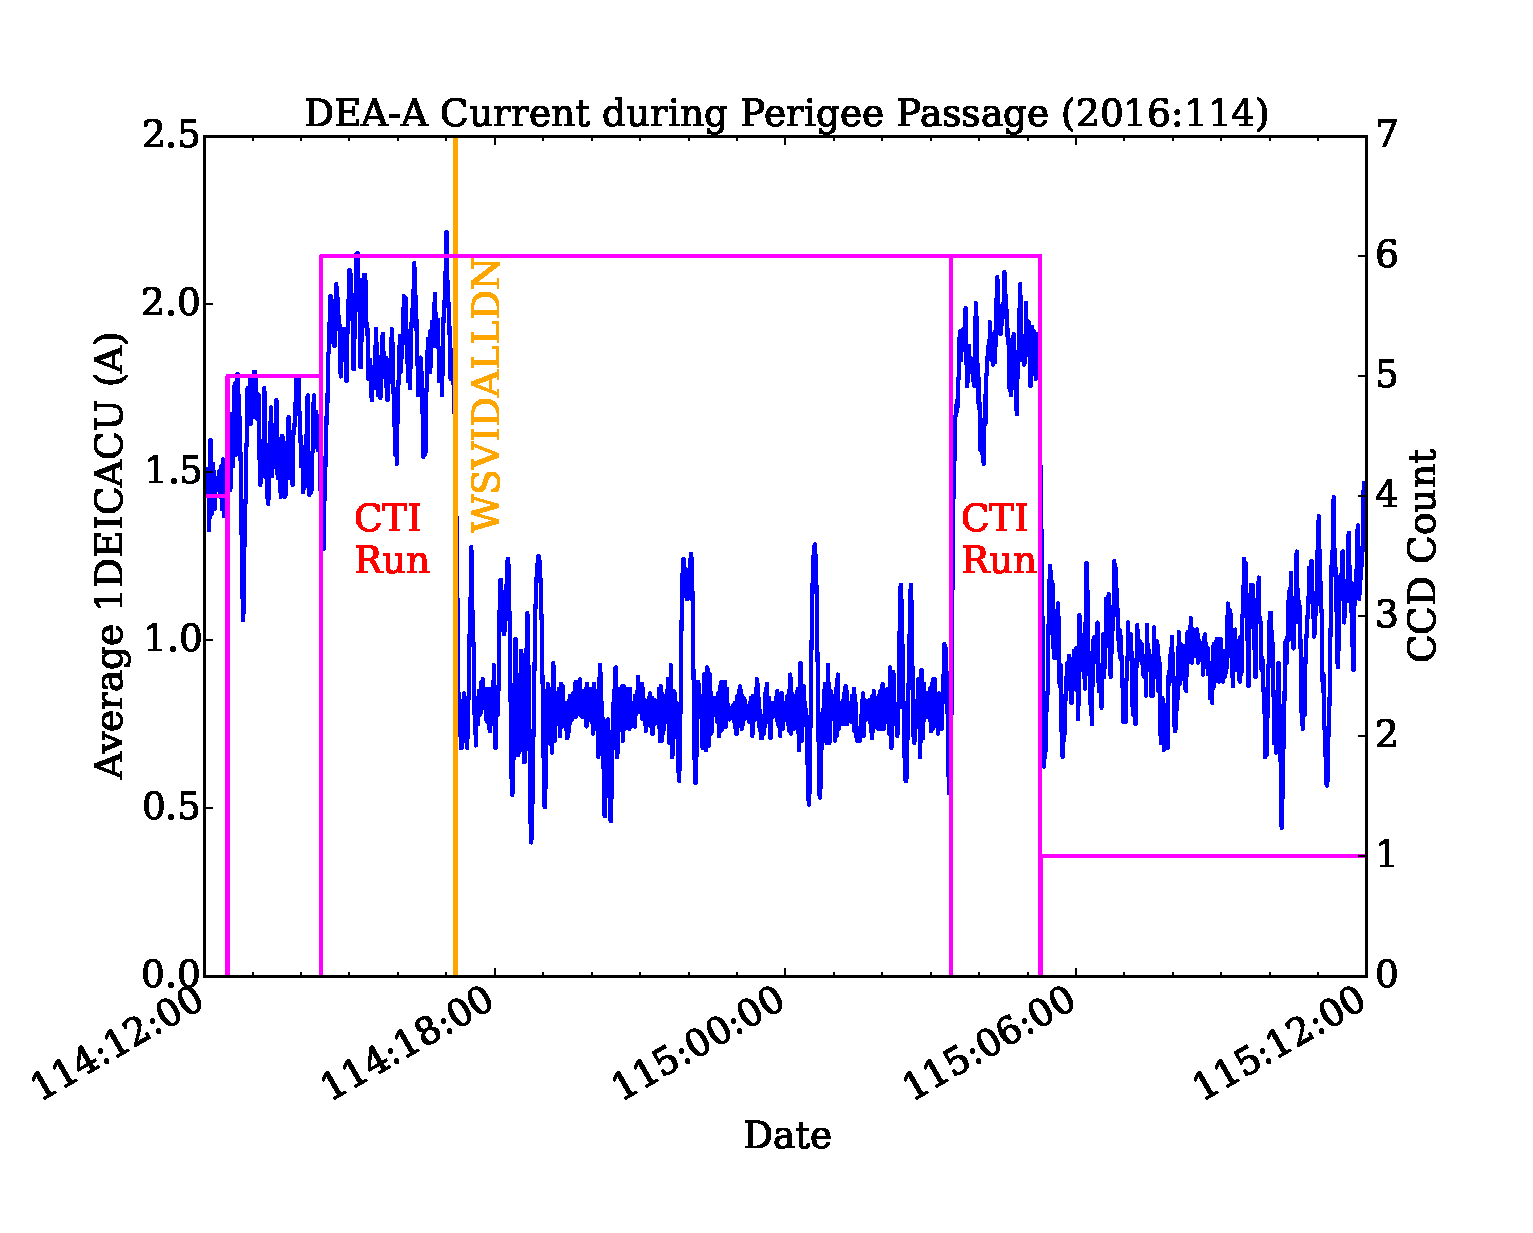
\includegraphics[width=1.2\textwidth]{switch_deaa_b_fig1.eps}
\caption{Average behavior of 1DEICACU during a perigee passage. All video boards
are powered off after the issuing of the WSVIDALLDN command, which is marked by
the orange line in the plot.}
\end{center}
\end{figure}
\end{landscape}
  
\begin{landscape}
\begin{figure}
\begin{center}
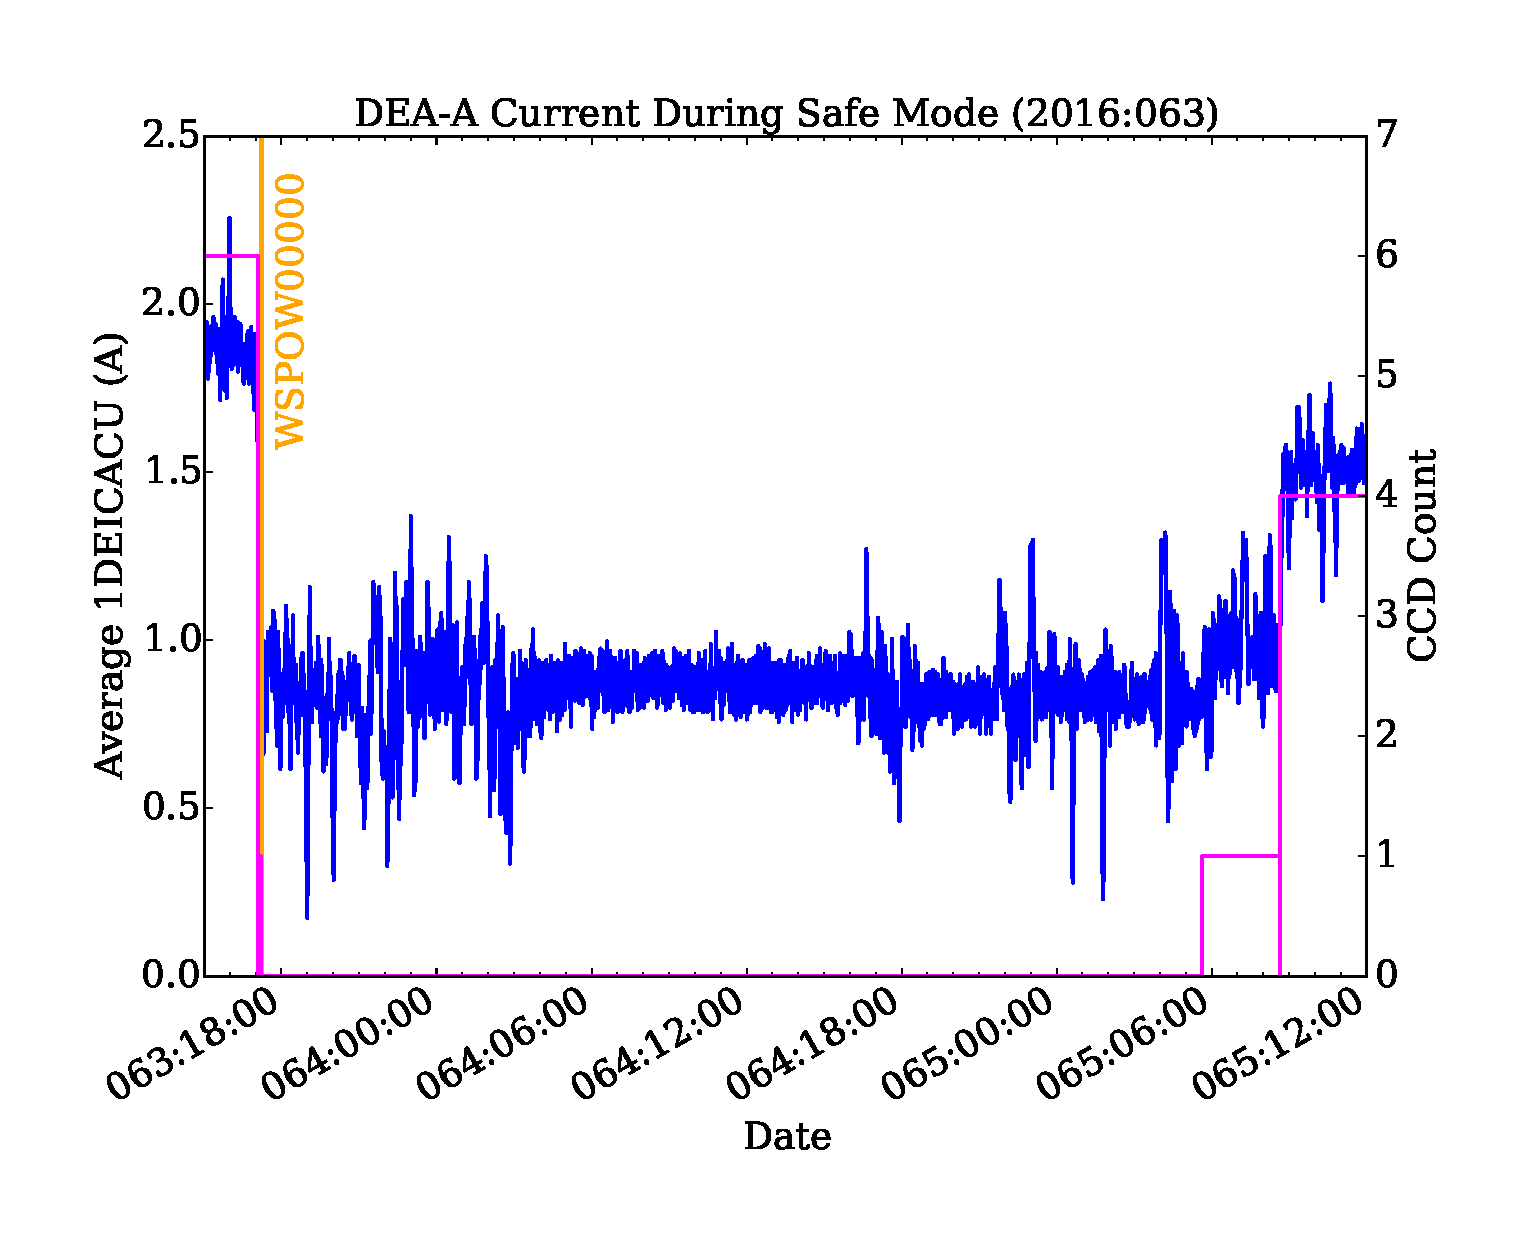
\includegraphics[width=1.2\textwidth]{switch_deaa_b_fig2.eps}
\caption{Average behavior of 1DEICACU during a safe mode. All video boards
are powered off after the issuing of the WSPOW00000 command, which is marked by
the orange line in the plot.}
\end{center}
\end{figure}
\end{landscape}
  
\newcommand{\tablecaptiontext}{SWITCH FROM DEA A TO DEA B}
\documentclass[11pt]{article}

\usepackage{lscape,color}
\usepackage[normalem]{ulem}
\usepackage{url}
\usepackage{graphicx}

\topmargin -0.75truein
\oddsidemargin -0.4truein
\textheight 9.25truein
\textwidth 6.7truein
\hbadness=10001
\hfuzz=200pt

\begin{document}
\newcommand{\be}{\begin{enumerate}}
\newcommand{\ee}{\end{enumerate}}
\newcommand{\bc}{\begin{center}}
\newcommand{\ec}{\end{center}}
\newcommand{\bi}{\begin{itemize}}
\newcommand{\ei}{\end{itemize}}
\newcommand{\bd}{\begin{description}}
\newcommand{\ed}{\end{description}}
\newcommand{\bt}{\begin{tabbing}}
\newcommand{\et}{\end{tabbing}}
\newcommand{\eg}{{\it e.g.~}}
\newcommand{\ie}{{\it i.e.~}}
\newcommand{\ul}{\underline}
\newcommand{\axaf}{{\em AXAF}}
\def\la{\hbox{\rlap{$<$}\lower0.5ex\hbox{$\sim$}\ }}

\centerline{\large {\bf 5.9\_V2.2 SWITCH FROM DEA A TO DEA B }}
\vspace{0.25in}

\noindent{\it Last Revised: December 6, 2017}\\
\noindent{\bf Filename: switch\_deaa\_b} \\


\noindent{\bf BRIEF FUNCTIONAL DESCRIPTION:}\\

This is a contingency procedure to switch from powering the DEA 
from the side A power supply board to the side B power supply board inside 
the PSMC. After switching DEA input power and reestablishing control of the
focal plane heaters, the magnetic relays that control pairs of video boards 
are thrown one at a time, and those two video boards are powered up separately,
while verifying that the PSMC doesn't report a current overflow.

Once 10 video boards have been powered up, power up 6 FEPs and execute bias-only 
runs in the ACIS-I and ACIS-S configurations to generate accurate video-board 
housekeeping. Once finished, power down all FEPs and video boards.

\vspace{0.15in}

\noindent The sequence of actions will be:
\begin{itemize}
\item Power down the video boards (skip if not powered)
\vspace{-0.10in}
\item Turn off and disable the DEA side A power supply (skip if not enabled and on)
\vspace{-0.10in}
\item Verify that DEA side A is off and disabled
\vspace{-0.10in}
\item Verify that all DEA side B heaters are off and disabled
\vspace{-0.10in}
\item Enable and turn on the DEA side B power supply
\vspace{-0.10in}
\item Verify that DEA side A is off and disabled
\vspace{-0.10in}
\item Perform a warm boot of the active BEP
\vspace{-0.10in}
\item Start DEA interface housekeeping
\vspace{-0.10in}
\item Enable DEA-B to assume control of the focal plane temperature
by commanding it to $-122^\circ$~C and then to $-120^\circ$~C
\vspace{-0.10in}
\item Switch the video board relays one at a time,
wait for PSMC telemetry verifiers to refresh,
and verify that DEA-B hasn't powered down due to an overcurrent
or overvoltage condition
\vspace{-0.10in}
\item After switching each pair of video boards,
power up each of the two boards, waiting for PSMC telemetry verifiers to 
refresh, and verifying that DEA-B hasn't powered down due to an overcurrent
or overvoltage condition
\vspace{-0.10in}
\item Power up 6 FEPs
\vspace{-0.10in}
\item Execute a bias-only science run in the ACIS-I configuration.
\vspace{-0.10in}
\item Execute a bias-only science run in the ACIS-S configuration.
\vspace{-0.10in}
\item Power down all FEPs and video boards
\vspace{-0.10in}
\item Dump the system configuration table
\end{itemize}

\vspace{0.15in}

\noindent{\bf ASSUMED INSTRUMENT STATE:}
\bi
\item Assumes that DPA A and/or DPA B is on, the flight SW is running and no 
science run is in progress.
\ei

\vspace{0.15in}

\noindent{\bf SPECIAL INITIAL CONDITIONS:}
\bi
\item Assumes that telemetry is in Format 1 or 2.
\item Assumes that neither the bakeout heater nor the detector housing heater is
being powered by DEA-B. If they are, switch them off and, if the procedure ends
with the DEA powered from DEA-B, consider enabling and turning them on again
on DEA-A.
\ei

\normalsize
\noindent {\bf OPERATIONAL CONSTRAINTS/CAUTIONS:} \\
\normalsize

In normal operations, only one side of the DEA should be powered on
(a) to prevent conflict for control of the focal plane temperature controller,
(b) to avoid excess current draw from the spacecraft,(c) to avoid over-heating
within the PSMC, and (d) to avoid placing a board 11 or 12 relay into the 
``magnetic neutral position''.

The DEA power status is normally indicated by the values of the 1DEPSA and
1DEPSB flags, which should not both be 1 simultaneously. Before sending the 
command to power on DEA B, the DEA Input Voltage B 1DE28BVO should 
be checked to make sure that DEA B is receiving power from the spacecraft.

The DEA input current monitors (1DEIC[AB]CU) are noisy.
To give an indication of what variation may be expected, figures 1 and 2
show the behavior of the A-side DEA current with a ten-sample running
average for two situations in which all video boards were powered down. Note that
when either side of the DEA is unpowered, the corresponding current monitor, 
1DEICACU for side A, or 1DEICBCU for side B, will be unreliable. They will read
16--18~A when unpowered, as of Telemetry Database (TDB) v14. This is expected and
not a problem.

If the DEA powers off unexpectedly during a bakeout, the FP bakeout 
heater will lose power and this heater will NOT be re-enabled when the DEA side B 
power is restored. Additional SW commands are necessary to activate the FP bakeout 
heater. The DH bakeout heater is unaffected by a power loss to the DEA and will 
therefore still be executing a bakeout if power is lost to the DEA.

The WSPOW commands in Step 8 of this procedure sequentially power up more and more 
video boards. Under some circumstances (e.g. looking for a board that may have a 
short or other anomaly), we may wish to skip one or more boards (e.g. suspected 
short circuit or other problem on one board). 

For more information about the relays, the DEA relays memo at 
\url{http://cxc.cfa.harvard.edu/acis/memos/DEA_Relay_Summary.html} should be 
consulted.

The parameters for the threshold crossings patch, txings, will revert to defaults 
when this is run. They should be restored to their desired values.

After successful execution, {\em the FP temperature control will be regulated at 
-119.7~$^\circ$C (if the spacecraft thermal environment allows), and DEA interface 
A/D will be in high-resolution mode.}

Skipping one or more boards in the power up sequence would require different 
WSPOW commands than are currently in this procedure.

Should any of the parts of step 8 fail or be intentionally skipped, so that less 
than 10 video boards remain powered up at the start of step 9, it will not be 
possible to obtain correct housekeeping from any of the video boards, so steps 
9-12 should be omitted.
\\

\newpage

\noindent{\bf CHANGE HISTORY:}

\bd
\item {\bf Version 1.2}
\bi
\item added a new step 1 to start a DEA HKP run if necessary
\item changed HW TLM verifiers to check state of DEA A and DEA B in
steps 2.1 and 3.2
\item added a new step 5 to warmboot the active BEP
\item added a command in step 6 to set the focal plane temperature to
$-120^\circ$~C
\item added operational constraint/caution that the B side does not
produce the telltales to verify the state of the relays
\ei

\item {\bf Version 2.0}
\bi
\item ACIS Team signed-off version
\item changed expected value of ``1STAT7ST'' in step 5.6
\ei

\item {\bf Version 2.1}
\bi
\item changed comment in step 1.2 to read ``check FP temp''
\item changed telemetry verified in step 5.5 to read ``version=??''
  and changed comment to read ``version \# depends on loaded patches,
  if any''
\item changed expected value of ``1STAT7ST'' in step 5.6
\item changed command in step 6.2 to WSFTNEG121
\item added to ``Assumed Instrument State'', ``Assumes DEA A is on''
\ei

\item {\bf Version 2.2}
\bi
\item added explicit steps to verify that DEA side A is off after sending the
disable and power off commands to side A and after DEA B is powered on
\item added explicit step to verify that the side B DH heater and the side B 
DH Bakeout heater are off before powering DEA-B
\item replaced command to switch all 5 relays simultaneously with 5 sets of 3 
commands: a command to switch one of the relays, followed by a pair of commands
to power up each of the two boards controlled by that relay
\item added command to power up 6 FEPs
\item added bias-only run to acquire housekeeping from ACIS-I boards
\item added bias-only run to acquire housekeeping from ACIS-S boards
\item added command to power down all video boards
\item added figures showing behavior of 1DEICACU
\item updated operational constraints and cautions text
and 
\ei
\ed

\begin{landscape}
\begin{figure}
\begin{center}
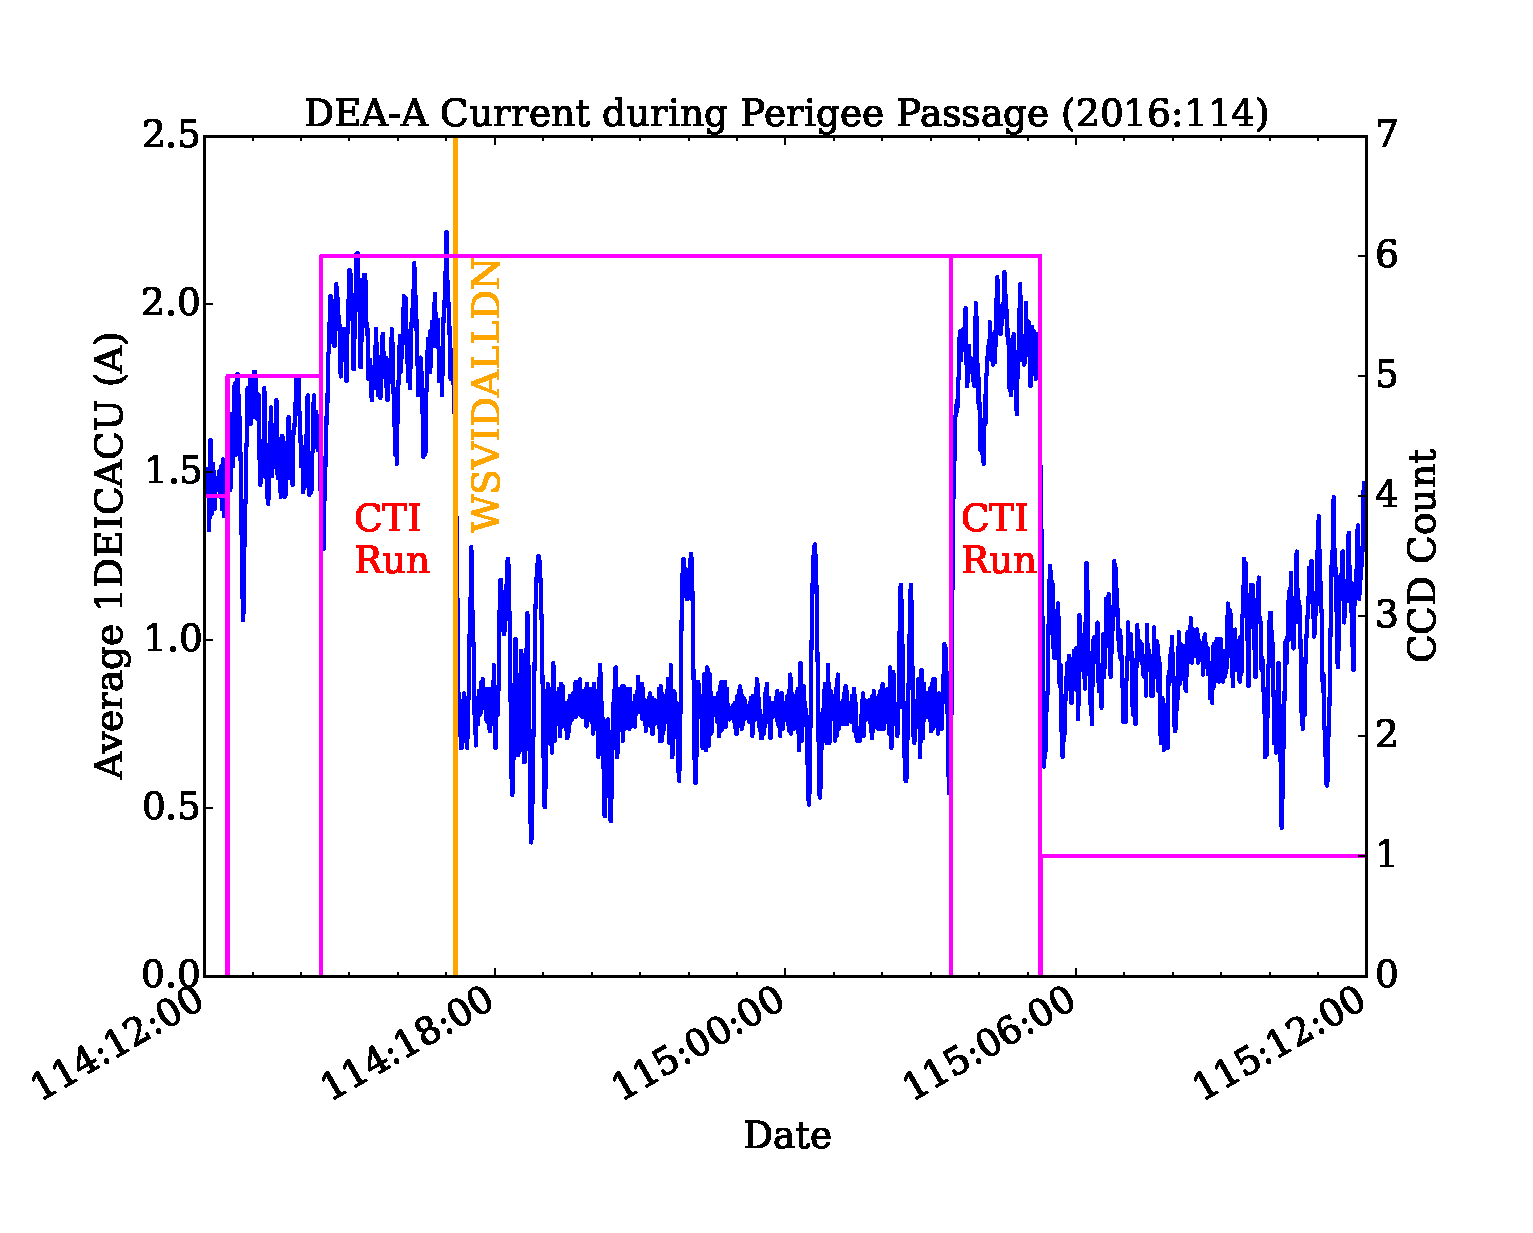
\includegraphics[width=1.2\textwidth]{switch_deaa_b_fig1.eps}
\caption{Average behavior of 1DEICACU during a perigee passage. All video boards
are powered off after the issuing of the WSVIDALLDN command, which is marked by
the orange line in the plot.}
\end{center}
\end{figure}
\end{landscape}
  
\begin{landscape}
\begin{figure}
\begin{center}
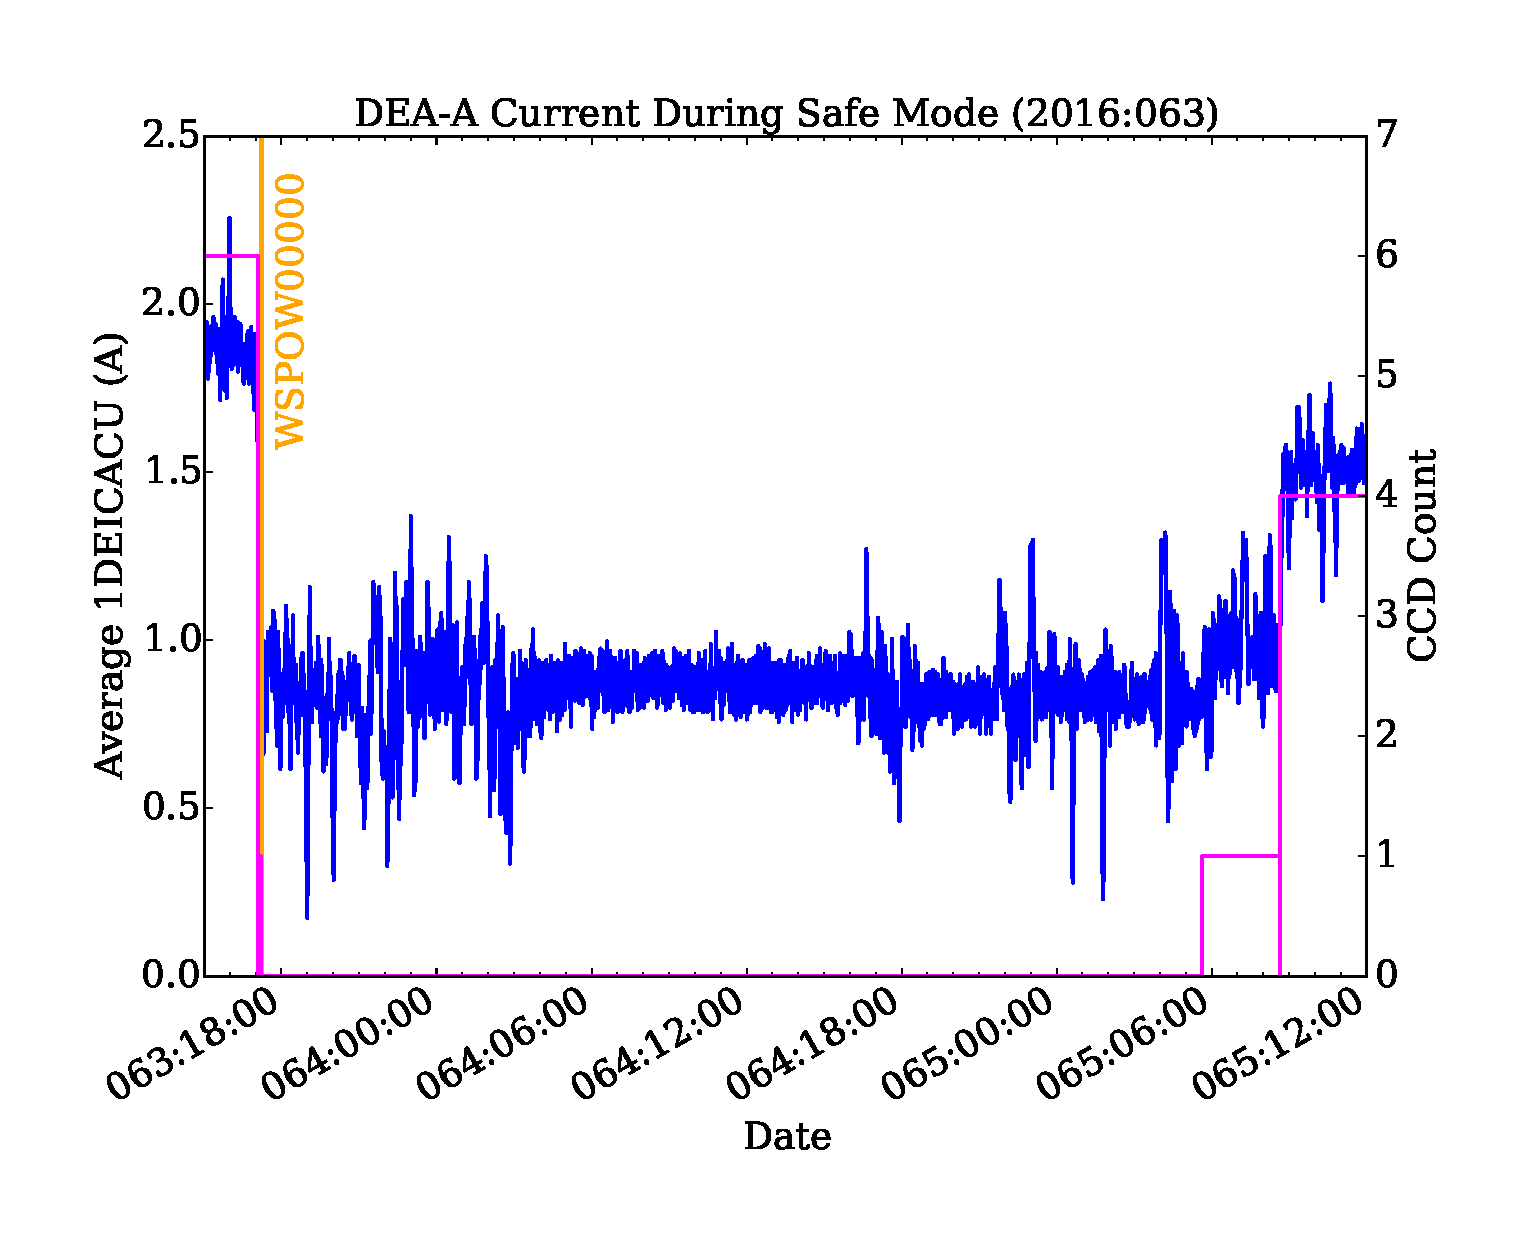
\includegraphics[width=1.2\textwidth]{switch_deaa_b_fig2.eps}
\caption{Average behavior of 1DEICACU during a safe mode. All video boards
are powered off after the issuing of the WSPOW00000 command, which is marked by
the orange line in the plot.}
\end{center}
\end{figure}
\end{landscape}
  
\newcommand{\tablecaptiontext}{SWITCH FROM DEA A TO DEA B}
\input{switch_deaa_b.tab}

\end{document}


\end{document}


\end{document}


\end{document}
